\documentclass[a4paper,10pt]{article}



\usepackage{listings}
\usepackage[english]{babel}
\usepackage{graphicx}
\usepackage[colorlinks, linkcolor=black, citecolor=black, urlcolor=black]{hyperref}
\usepackage{geometry}
\geometry{tmargin=3cm, bmargin=2.2cm, lmargin=2.2cm, rmargin=2cm}
\usepackage{todonotes} %Used for the figure placeholders
\usepackage{ifthen}


%=== TITLE & AUTHORS ====================================================================
\begin{document}

\title{Execution models}
\author{Maria I. Artigas}

% The paper headers
% \markboth{IEEE TRANSACTIONS ON MICROWAVE THEORY AND TECHNIQUES, VOL.~60, NO.~12, DECEMBER~2012
% }{Roberg \MakeLowercase{\textit{et al.}}: High-Efficiency Diode and Transistor Rectifiers}


% ====================================================================
\maketitle



% === ABSTRACT ====================================================================
% =================================================================================
\begin{abstract}
%\boldmath

\end{abstract}


% === KEYWORDS ====================================================================
% =================================================================================


% ====================================================================
% ====================================================================
% ====================================================================


% === I. INTRODUCTION =============================================================
% =================================================================================
\section{Introduction}

This document aims to explain the methods for coordination of resources in the context of Assembly Execution System in AssemblyRecon and an assembly case in PROUD. The structures presented here aim to help representing and coordinating the execution of multi robot tasks,  with time extended assignments and multi task robots according to the classification in \cite{korsah2013comprehensive}. 

%Small introduction on how the purpose of this report is to make a link between declarative constraints among tasks and resources, with the coordinated execution of them given the resource-task allocation.

\section{Task dependency relations }


A minimal set of relations is presented in this section for structuring partial task specifications.  This relations aim to provide needed dependencies on what has to be done, using which capabilities.
%As previously mentioned, the declarative structure presented aim to provide a base to declare multi robot tasks, with extended assignments and multi task robots. 
For this purpose, the set of relations for the task specification should also allow linking task specification with the resource capabilities required for execution.
The set of relations can be divided in two major sets: task interdependencies, and dependencies between task and capabilities of resources. % RETHINK IF MENTIONING RESOURCES OR CAPABILITIES, AS YOU ARE DOING THE SWITCH WITHOUT PREVIOUSLY MENTIONING THE LINK

The data structure used to store task specification in this work is linked data. This is due three main reasons:
\begin{itemize}
    \item Flexibility to link different types of data, independently of content or granularity. (This allows to perform similar methods of decision making on different levels of granularity of the data).
    \item Flexibility of internal structures. As it is based on triples, internal structures do not constraint the linking of data.
    \item Accessible entry to the data through semantic queries.
\end{itemize}
%ADD EXAMPLE OF GRAPH
\subsection{Task interdependencies}
% MAKE THE RIGHT CITATION

%Cyber-physical systems tasks can % are defined and constraint by dependencies among tasks and other situation information
% In cyber phisical tasks are continuous on time, which is why their performance has as key character its duration
% for this reason, when having contraints between tasks, the duration characterization has to be taken into account.
The temporal side of task dependencies can be described from interval theory representations \cite{1}.
From this work the temporal interval relations to be inherited are (see figure \ref{fig:allens_framework}): \\
$\{ before ,meets ,overlaps ,starts ,during ,finishes ,equal \}$.
\\
\begin{figure}[h]
    \centering
    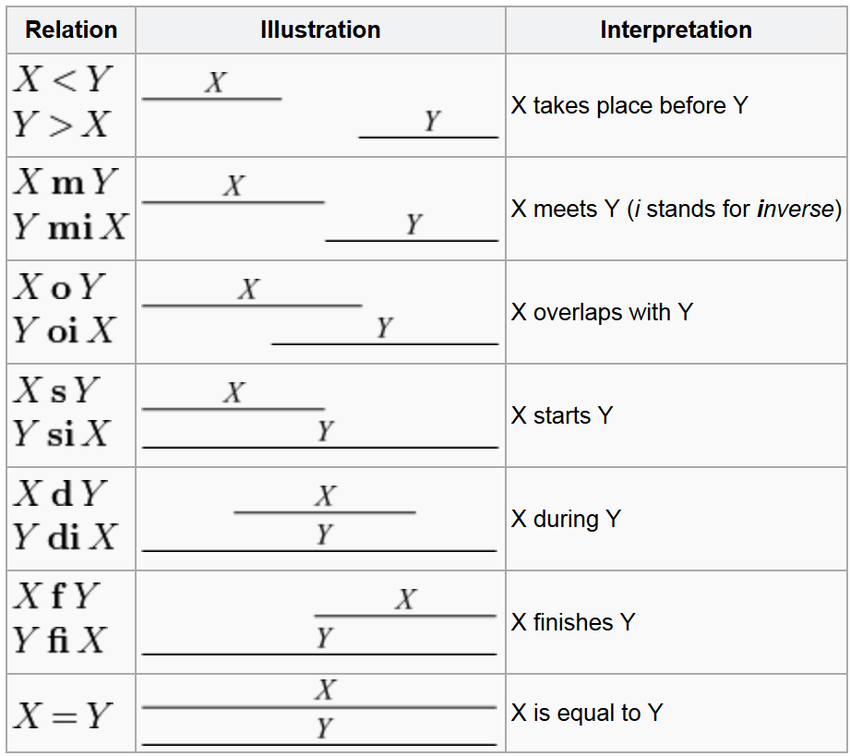
\includegraphics[width=0.5\textwidth]{allens_framework.png}
    \caption{Allen's framework relations}
    \label{fig:allens_framework}
\end{figure}


%ADD THAT TO INTRODUCE TIME DEPENDENCY CONTRAINTS YOU NEED TO DEFINE WHICH PART OF THE RELATION HOLDS THAT DEPENDENCY
The task can be expressed as a set of subtasks which are interrelated with the previous relations in a directed manner. According to the definition in \cite{1}, we can appreciate that the definition of direction of the relation indicates the precedence between the tasks, aside from the equal relation. The equal relation can be defined as bidirectional there is no precedence among the tasks.
\\
These categories only cover the overlapping of tasks. How and who imposes the dependency complements the previous information when coming to execution methods.  
% Add example
To this work, the concept of necessity has to be added. Who needs this relation to hold? 
For example, task a and b can be equal. When perform task a, task a needs task b to be performed at the same time (equal relationship). However, task b might not need task a to be performed simultaneously. For example, to move a rotor (task a) we need the gripper to be actively closed (task b), but the gripper can be actively closed also in other situations not including the performance of moving the rotor. 
\\

When taking the subgraph from the task composed by the nodes which are related by before relation, this subgraph is a directed acyclic graph. The cause of this is the requirement on the lack of loops in the execution. 
The composed graph (with the other relations included) allows the expression of different paths to execute the same task, which composes a more robust execution, given the choice of different executions for the same task. % Reformulation needed

\subsection{Dependencies between task and capabilities of resources} 

The execution of these tasks can be realized by a set of capabilities of the resources. 


From the point of view of execution of tasks, the minimum relations needed for the characterization of the resources (active) % CHECK IF IT ALSO HOLDS FOR PASSIVE RESOURCES
are the mereological (check) description of the resources (to define different levels of hierarchy in the resource control and allocation) and the topological description of the resources available (to define the attributes and capabilities of the resources in the context of control and allocation). This data forms the base information for checking the feasibility of tasks and their following allocation.

% Introduce the tree structure over capabilities
% Introduce the relation with the particular resources
% Introduce the relation to the category of resources


The link between the task and the resources is defined by the capabilities which can provide the task. In the paradigm of linked data, this is represented as the relation %{FILL ME IN}
% You can describe that the good thing of this description is good as you can do it at any level of granularity of capabilities or part in the resource tree, but I find it redundant with the introduction on link data, though you can mention it on the examples part


\subsection{PROUD: Skill Execution Graph}

For demonstration of the previous approach, an illustration case is the assembly of an snapfit. In this case, the resource available is a industrial arm manipulator with a gripper as end effector.

For the execution models required the task interdependencies can be defined as a graph containing the different paths for the execution of the assembly (see figure \ref{fig:assembly_dag} ). In this representation, the different routes over the graph, from the start subtask to the finishing subtask have the meaning of a mode of execution.

\begin{figure}[h]
	\centering
	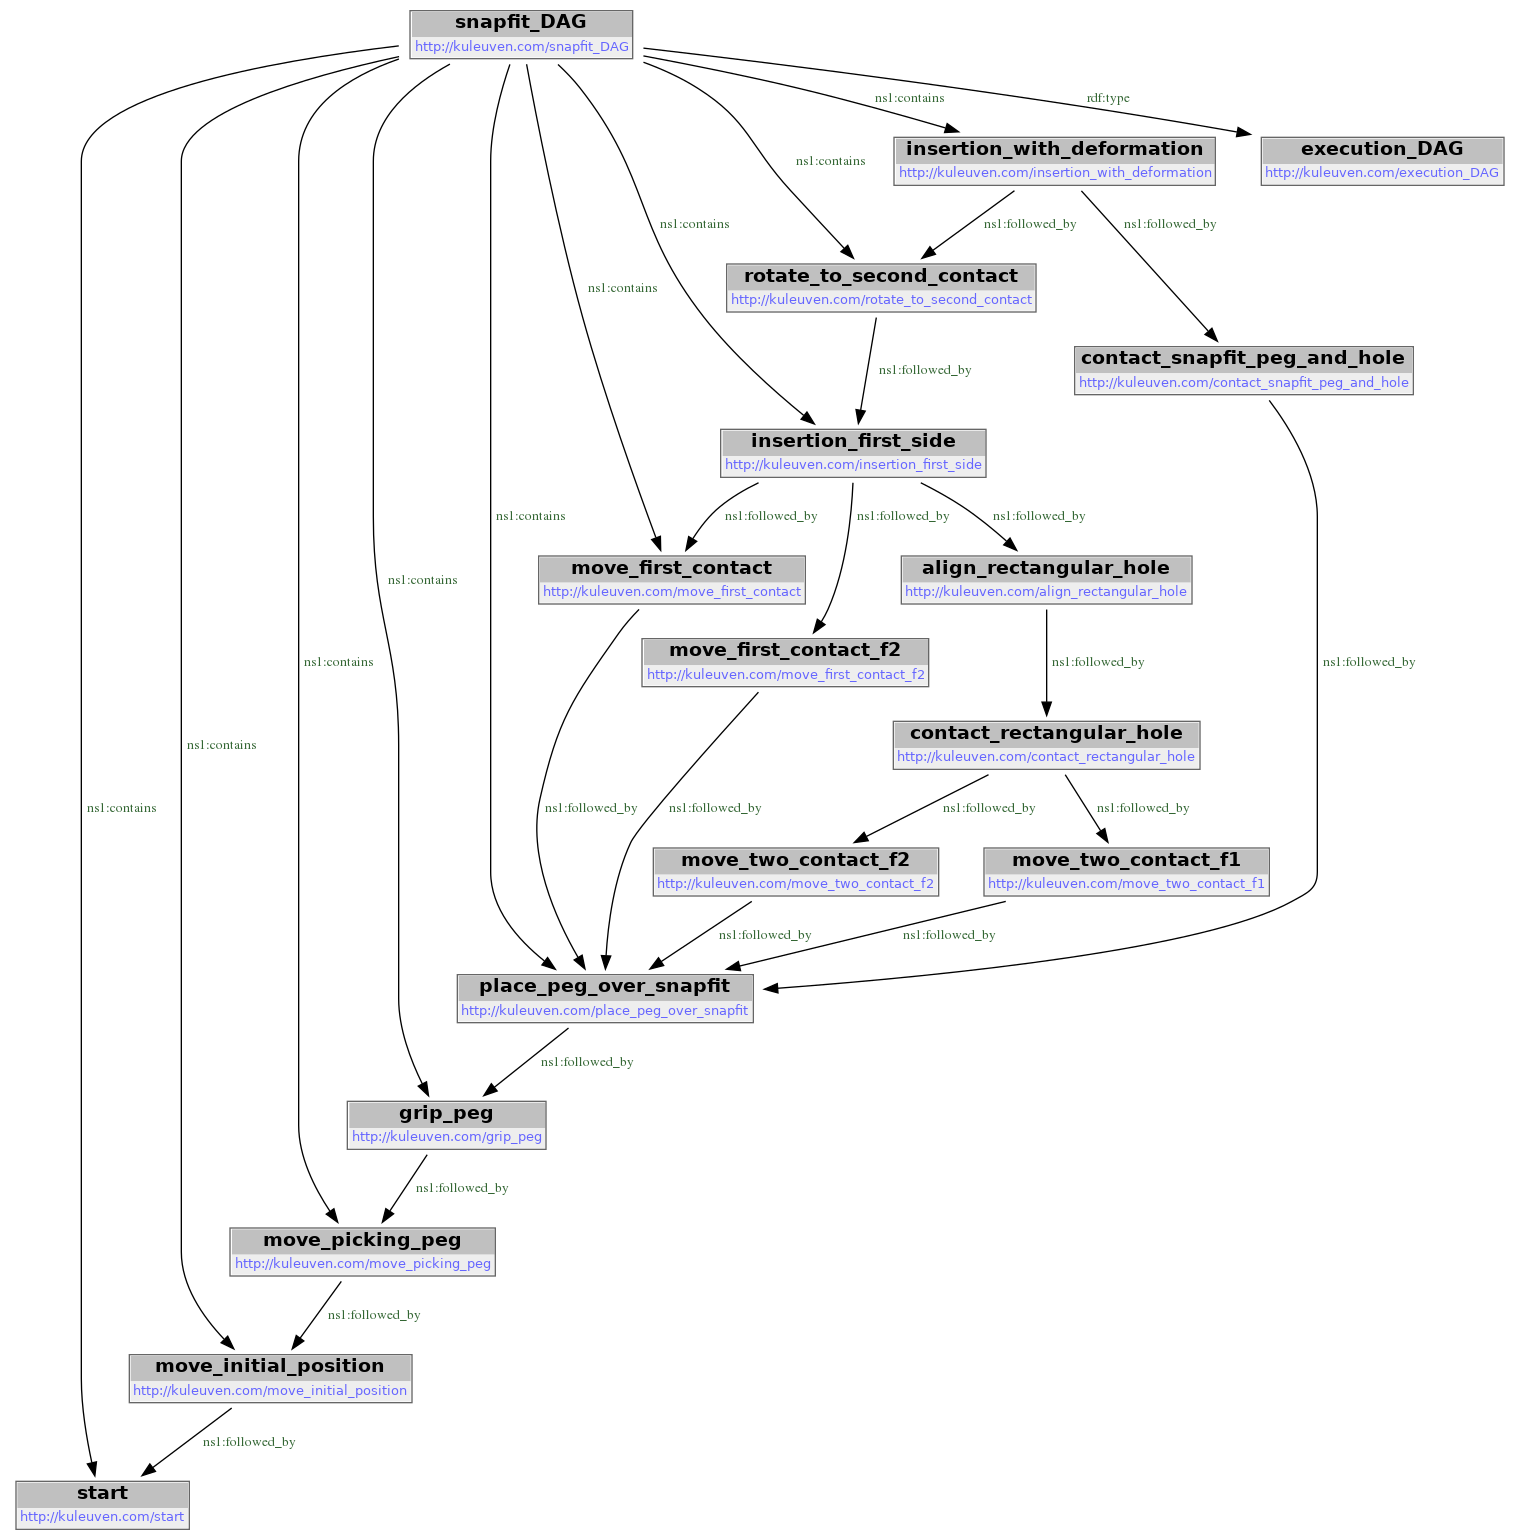
\includegraphics[width=0.5\textwidth]{snapfit_dag.png}
	\caption{Allen's framework relations}
	\label{fig:assembly_dag}
\end{figure}


\subsection{AssemblyRecon: Product Execution Graph}

AML /ISA 95 and translation to these concepts

Task + resource = skill for the resource

Assembly graph 

The transition tasks in the model are described as:

\begin{figure}
\begin{lstlisting}

  {
    "@id": "http://kuleuven.com/grip_rotor",
    "http://kuleuven.com/needs_precondition": [
      {
        "@id": "http://kuleuven.com/move_to_rotor"
      },
      {
        "@id": "http://kuleuven.com/rotor_visual_check"
      }
    ],
    "http://kuleuven.com/needs_capabilities": [
      {
        "@id": "http://kuleuven.com/move_cartesian"
      },
      {
        "@id": "http://kuleuven.com/visual_check"
      },
      {
        "@id": "http://kuleuven.com/grip"
      }
    ]
  }
\end{lstlisting}
	\label{fig:assembly_recon_task}
\end{figure}

This representation of the task differs to the one in the previous case in the meaning of the connection among subtasks. In the case presented in \ref{fig:assembly_recon_task}, the relationship $/needs\_precondition$ explicitly defines the dependency of the subtask over all the subtasks it is related.This means the need of all the preconditions to be previous to the task. In the case presented  in \ref{fig:assembly_dag} the relationship $/followed_by$ describes the different paths in which the pre-dependencies of a task can be fulfilled.  

%Task interdependencies example:

%Bill of materials:


%Bill of resources:

%Capabilities of resources: 

%CONTINUE MODEL WITH PAGE 219 -> DUAL LEVEL TASK SPECIFICATION: GUARDED ORDER EXECUTION 


\section{Task dependency model to task execution model}

Given the task specification as the structure presented in the previous section, the next step towards execution, is the connection to required coordination models.

Every task (which was represented as a subgraph or node in the previous section), should be composed with the resource capabilities information in order to compose the coordination required for its execution. This composition is developed with 2 types of models in this work: finite state machines and petri nets.

\subsection{Task dependency model to task execution model: Petri net coordination}


Petri nets are chosen as coordination method. For it, the main aim is to translate the declared dependencies between task-task and task-resource to the petri nets. As result, the petri net contains the required information for synchronized work of shared resources.\\

%ADD SMALL DESCRIPTION OF PETRI NETS 

The model of our petri nets contains a translation from a task dependency graph as executable graph. 
Tasks are modelled as 2 places in the petri net. The "start" place is to be filled with a token when the task is ready to start, while the "wait" place is filled in when the task is done.
The places representing the task are complemented by two transitions, the "start" transition and the "end" transition. The "start" transition will be triggered when all the dependencies for starting the task are fulfilled. The end transition is trigger when the task is finished. To avoid inconsistencies, the "end" transition is also connected to the start place of a task, to not allow the finishing of a task before its own start. 
The previous representation of task in the petri net is illustrated in \ref{fig:task1_petri}.

\begin{figure}[h]
    \centering
    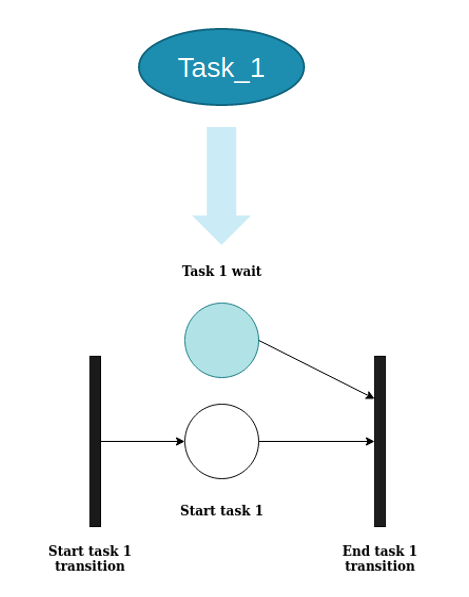
\includegraphics[width=0.3\textwidth]{task1_petri.png}
    \caption{Task representation in petri net}
    \label{fig:task1_petri}
\end{figure}


To represent precondition dependencies in the petri net a place is added as intermediate condition (see figure \ref{fig:pre_petri}). This allows to force the fulfilling of the precondition task before, as setting its performance as a condition to trigger a secondary task. 
\begin{figure}[h]
	\centering
	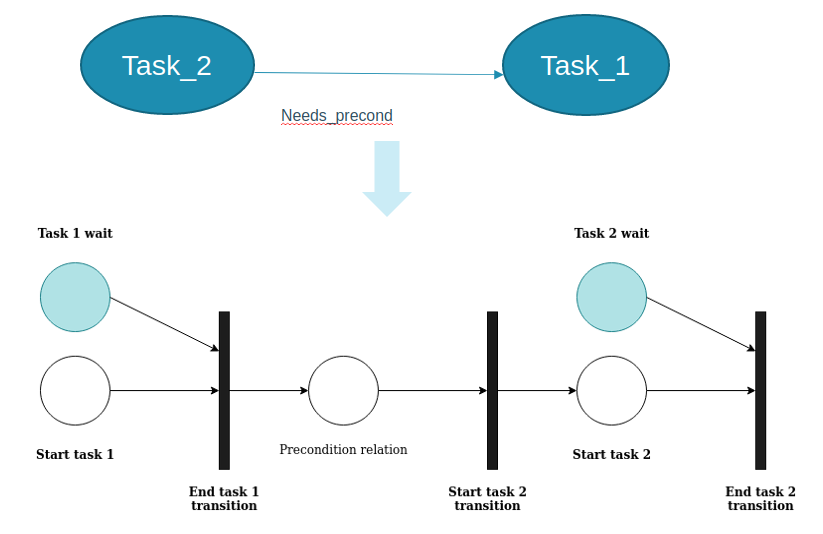
\includegraphics[width=0.3\textwidth]{precondds.png}
	\caption{Task preconditions in petri net}
	\label{fig:pre_petri}
\end{figure}

To represent n resource dependencies of the task, n+1 places will be added to the petri net. N places will represent the commitment of the resource to the task for the duration of the task. When all resources are available for the task (resource places have a token), an intermediate trigger (as shown in the figure \ref{fig:res_petri}) is triggered, denoting the commitment of all resources to that task. If the other places connected to the task "start" transition have a token, the start of the task can be triggered. 

\begin{figure}[h]
	\centering
	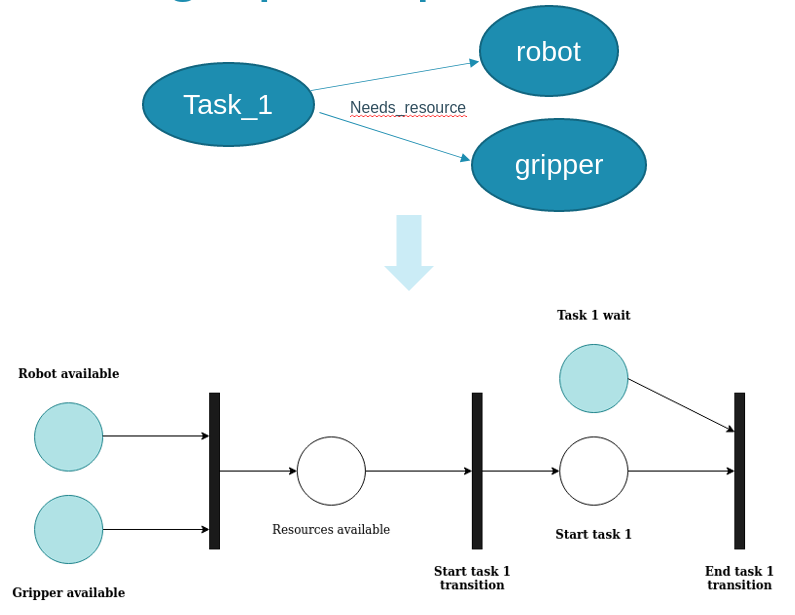
\includegraphics[width=0.3\textwidth]{resources_dep.png}
	\caption{Task-resource dependency representation in petri net}
	\label{fig:res_petri}
\end{figure}


% WRITE ABOUT FLAGS AND THE PETRI NET MEDIATOR WHICH CONTROLS THE PETRI NET


%This is because in the petri net, the granularity at the task/skill level is not relevant, given the flags and tokens are filled in accordingly.

%One petri net per task (one mediator per petri net)

%One communication channel per resource (one communication mediator per resource)

\subsubsection{PROUD: Skill Execution Graph}

\begin{figure}[h]
	\centering
	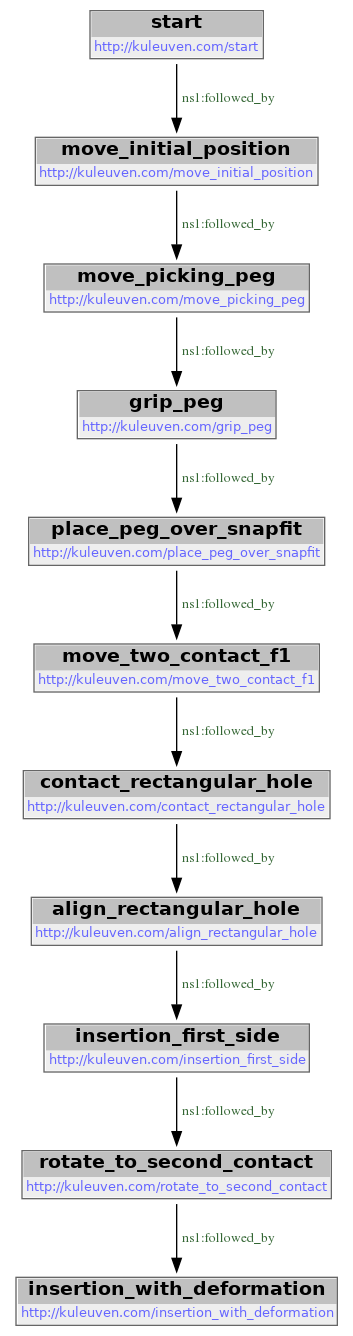
\includegraphics[width=0.2\textwidth]{0path.png}
	\caption{Snapfit case task path}
	\label{fig:snap_path}
\end{figure}

In the case of the execution graphs used for PROUD presented in \ref{fig:assembly_dag}, the relationship $/followed_by$ describes the different paths in which the pre-dependencies of a task can be fulfilled. For the previous conversion from execution dependencies to petri net, the graphs required must present the sequence of preconditions which need to be fulfilled to execute a task. This means the need of a decision making step from the model presented to an execution model as the one in \ref{fig:snap_path}.


\subsubsection{AssemblyRecon: Product Execution Graph}

In the case of AssemblyRecon, from the representation in \ref{fig:assembly_recon_task}, a direct conversion to the petri net can be applied. 

%\subsection{Task dependency to task execution models: LFSM reactivity}

\section{Stable states in petri nets and fsms}

The concept of stability can be defined as the lack of fluctuations or change of a property (or set of properties) 
Physical stability can be defined as "The ability of a product to maintain its physical dimensions and properties when exposed to conditions normally encountered in its service environment". This concept can be extrapolated to the lack of change or fluctuations of a property (or set of properties) within the state of the world.
%Connection to preemption

The views on stability in this work are focused on 4 types of dependencies
\begin{itemize}
	\item CAD/area level 
	\item Skill level 
	\item Part/subassembly level 
	\item Tool level 
\end{itemize}

Stability in the previous levels is also extended at an informational level for its usage within autonomous systems. In the sense that the uncertainty over the information we have is low enough to assume we can continue with execution.

The concept of stability in cyber-physical systems is complemented by the concept of preemption. 

\subsection{Stability at skill level}

The skills can be divided as blocks of skills from stable state to a set of stable state. These blocks are partial order sets of skills to be executed. The interruption of these blocks of execution implies the interruption in a non-stable task state. While executing these skills, we contemplate 3 options in case of disruption of the POS execution:

\begin{itemize}
	\item Forward: proceed with the set of skills remaining until next stable state.
	\item Backwards: apply "inverse" skills to go back to last stable state.
	\item Interrupt: preempt the task by leaving in a stable state different from the 
\end{itemize}

% MAKE EXPLANATIONS OF INITIAL STATE (BEFORE BLOCK OF SKILLS), FINAL STATE, AND THE TRANSLATION TO THE THREE DIFFERENT METHODS OF DISRUPTION IN THE PETRI NET WITH COMPOSITION METHODS 

% MAKE EXAMPLE OF block of skills from assembly recon

Stable state = informational and factual state in which the property is ready for preemption? 


\subsection{Stability at part dependency level (passive resources)}

Stability at part level denotes the lack of change of a set of pieces with respect to each other, conditional to the lack of manipulation of the parts. Within the context of assembly with autonomous manipulators, the stability is extended to an informational level. The informational level meaning the availability of relevant knowledge over the location and state of the parts, for its manipulation.

% Make example at the skill level -> when rotor is inserted is stable -> when rotor is manipulated by the manipulator it is not stable (though it is located in reference to the manipulator)

% Parts have to be inserted in a poisition in which they are not going to move, and the location is known by the system

\subsection{Availability at tool/resource dependency level (active resources)}

Stability at the resource level denotes a state in which the robot or system is  


%\subsection{Stability at CAD level}

%Stability of areas: you have the semantic areas and what reasoning comes in when in an assembly you have to allocate the semantic areas and what happens if an area becomes available or it stops being available.


%\subsection{Stability at product/task dependencies level}

\section{Progress metrics extracted from petri nets and fsms}

Flag copy per resource 
Node in the fsm


\section{Preemption/backtracking at the level of petri nets and fsms}

High order flags to be added to the petri nets = timeouts, active ...(lcsm states), highwater, lowwater 
Page on preemption reasoning from what I wrote in the notebook

\subsection{Preemption at resource/tool level}

At resource level, preemption from stable state of resources to a new stable state of resources, can be seen as a set of tasks or skills which allow the correct transition. 

\subsubsection{AssemblyRecon: Preemption at resource/tool level}

For stopping the execution of a task, only going forward with the task is allowed. So the petri net has to be continued until the next stable state. To denote this in the petri net and keep the execution state, the "wait" place of the last task which ocurred has to remain empty. This denotation will allow the continuity of the task, as soon as the resources can go back to the execution of the interrupted petri net and fill in the token, re-triggering the continuity of the petri net.

%MAKE IMAGE WITH TWO PETRI NET -> ONE STOPPED BY THE OTHER TASK, THEN EXECUTION OF THE OTHER PETRI NET -> THEN PREEMPTION BACK AND CONTINUING THE PETRI NET AGAIN
%FOR LEAVING A TASK -> BOTH RESOURCES AND PARTS HAVE TO BE SET IN A STABLE STATE, MAYBE ALSO SPACE  




\section{Skill table between petri nets for task/resource/skill correlations}

\section{Communication protocol (optional)}
Flags and communication information 

Metadata regarding association between communication protocol and petri net generation -> 


\subsection{AssemblyRecon: task-resource/skill table}

Also talk about where to keep the state of the tool in the resource holon and then doing the preemption accordingly


\section{Delay impact regarding preemption/backtracking/contingency plans/rush orders}
\textcolor{cyan}{Here -> need to talk about critical resources, how you can predict the cascading and so on and so forth}

\section{Conclusion}

\section{Notes}

Make references to petri net plans (from https://sites.google.com/a/dis.uniroma1.it/petri-net-plans/publications?authuser=0) maybe in the introduction add the added value of this work over that. (Also as added value -> petri net mediator and flags -> make connections automatically with the agents instead of the agents having to keep up with the petri net)


\section*{Acknowledgment}

\bibliographystyle{abbrv}
\bibliography{bibliography.bib}
\end{document}



